\section{\name Compiler Overview} \label{sec:compileroverview}

In this section, we introduce the compiler framework---\name---that targets Plasticine
architecture from high-level programs described in the Spatial language. 
There are two challenges to map Spatial applications to Plasticine. 

First, unlike an FPGA, Plasticine cannot map arbitrary RTL functionality.
In the Spatial abstraction, the execution order of the program is organized by a control hierarchy, where
each level of the controller schedules the execution of the next level controllers.
When mapping the example in \Cref{fig:spatialegpar} onto an FPGA, the outer controller \emph{A}
sends an enable signal to each child controller, which signals back the parent controller when
completed. If the user chooses to sequentially execute the outer loop \emph{A}, the parent
controller enables the child controllers one at a time; if the user chooses to metapipeline
(coarse-grain pipeline) the outer loop \emph{A}, the outer controllers enables multiple child controllers in a pipelined fashion.

\begin{figure*}
\centering
  \centering
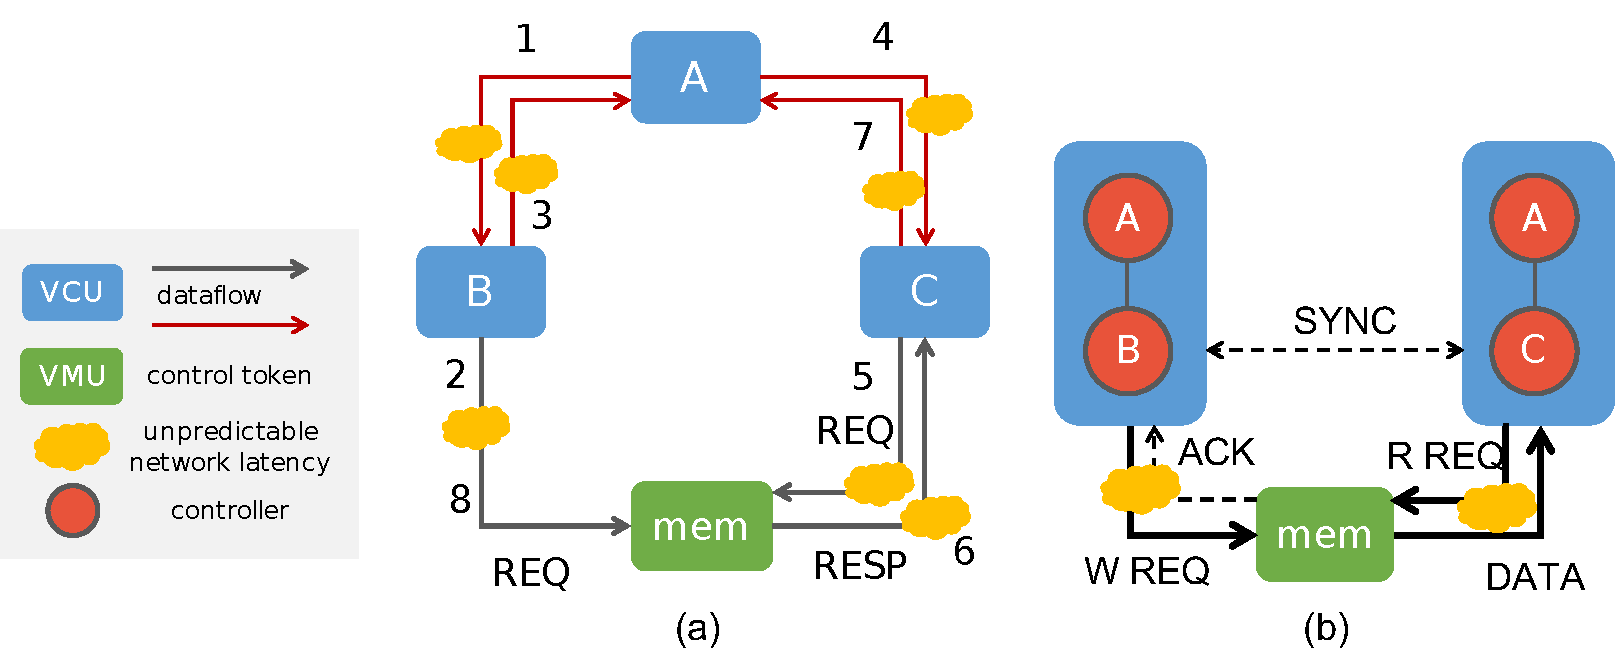
\includegraphics[width=0.8\textwidth]{figs/centralctrl.pdf}
  \caption[A na\"ive mapping strategy and distribute control flow in \name]{
  (a) A na\"ive mapping strategy to map the control hierarchy onto Plasticine.
  All units are distributed across an on-chip network that can introduce unpredictable latency.
  The number on the edges indicates event order.
  Here we show a scenario where read requests from \emph{C} do not observe the write requests from
  \emph{B} that occur earlier in the program order due to network latency between \emph{B} and
  \emph{mem}.
  (b) Distributed controllers in \name. Each innermost controller makes a copy of all enclosing controllers. The signals from these controllers are used to generate synchronization between distributed compute units. To address the problem in (a), the memory also needs to provide a write acknowledgment per write request for synchronization.
}
\label{fig:centralctrl}
\end{figure*}

To achieve the same execution schedule on Plasticine in a na\"ive approach, 
we can map each controller in the hierarchy into a PU, sending control signals to schedule the next
level controllers distributed among other PUs, as shown in \Cref{fig:centralctrl} (a).
This strategy suffers from the expensive network round-trip delays between the parent and child controllers.
To be scalable at a high clock frequency, Plasticine networks are pipelined at each switch,
introducing multiple cycles of network delay across PUs on the control path.
Therefore, the multi-cycle handshaking signals can lead to significant pipeline bubbles that undermine performance.
Additionally, this scheme creates a communication hotspot around the parent controller \emph{A} as
loop \emph{A} gets unrolled, which is devastating for a CGRA
like Plasticine that has much less routing resource than an FPGA.
Furthermore, synchronizing the compute only is insufficient to ensure memory effects are observed by
the remotely distributed accessors, as shown in \Cref{fig:centralctrl} (a).

To address this challenge, we want to eliminate centralized outer controllers.
At high-level, \name performs \term{loop divisions} on each outer controller, such that
all innermost controllers are perfectly nested, as shown in \Cref{fig:centralctrl} (b).
\Cref{sec:loopdiv} discusses the loop division transformation.
\name then allocates synchronization tokens across the distributed innermost controllers.
All innermost controllers have their own copies of the outer controllers, which are used to
generate the control tokens.
These control tokens ensure the execution order of the inner controllers is the same as if they are
scheduled by a centralized outer controller. Instead of synchronizing all inner controllers under an outer controller, \name only synchronizes the ones accessing the same memory, such as \emph{B} and
\emph{C} in \Cref{fig:spatialegpar}. This limits the synchronization among a small set of
distributed nodes without impacting the result, 
making our design much more scalable.

The second challenge is that controllers in the Spatial hierarchy
can consume an arbitrary amount of compute and memory resources, exceeding the capacity of individual
PUs. For instance, a user might write an on-chip memory multiple times throughout the program with writers
mapped to different PUs. The physical scratchpad, however, only has a single write port and write address
pipeline. 
\name maps a subset of the address computation externally in other PUs and generates control tokens among the distributed writers, time-sharing the write port, and enforcing the
ordering between distributed writers.
Using resource virtualization, \name composes or time-share the physical resources when software usage exceeding the hardware limit.

\begin{figure*}
\centering
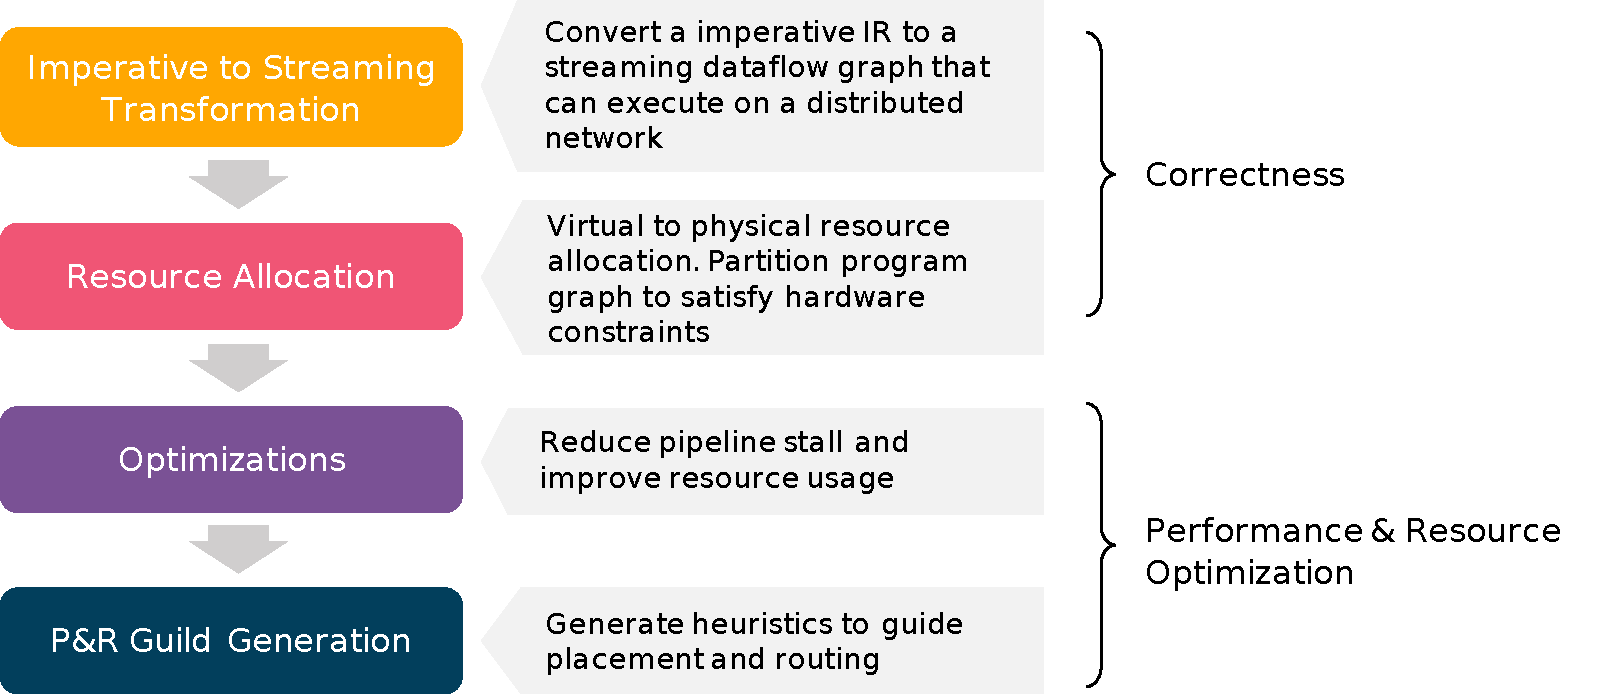
\includegraphics[width=1\textwidth]{figs/sarastack.pdf}
\caption[\name compiler flow]{\name compiler flow}
\label{fig:flow}
\end{figure*}
 
In the following sections, we describe a systematic approach to compile applications described in an
imperative front-end language to a purely declarative and distributed dataflow graph that can
run on Plasticine. \Cref{fig:flow} shows \name's compilation flow.

\Cref{sec:control} expands on the \term{imperative to dataflow transformation} that
addresses the first challenge.
\name allocates distributed on-chip resources to execute the program in spatially parallelized and
pipelined fashion with appropriate synchronizations.
A virtual unit (VU) is our intermediate representation that captures the computation mapped
within the boundary of a physical unit (PU), such as a PCU and PMU.
Each VU can contain multiple contexts if their aggregated resource usage can fit in a PU.
The hardware can limit the maximum number of contexts a PU can support and has resources that cannot be split across contexts.
Most importantly, \name needs to ensure messages across VUs, mapped across the global network,
tolerate an arbitrary amount of network latency; messages within a single VU across contexts takes only a single cycle.
The transformation phase generates a virtual unit dataflow graph (VUDFG) with appropriate
synchronizations, such that the parallelized and pipelined program executed over distributed on-chip resources produces the same result as a
parallelized program executed in time.
At the end of the allocation phase, a virtual unit can consume as many resources as the program
requires. 

\name further virtualizes resource allocation and hides the underlying resource constraints from the programmers.
\Cref{sec:resalloc} dives into the \term{resource allocation} phase, where \name assigns each VU to a
PU that processes the required resources. If no PU can fit a VU, \name partitions the
VU into multiple VUs to resolve the constraint violation. If there is insufficient PU or the VU cannot be partitioned, the mapping process fails with appropriate hints to the programmer for the
limiting resources.

Throughout the first two phases, \name introduces various \term{optimizations} that either reduce the
the resource cost of the VUDFG, or alleviate potential performance bottleneck in the streaming
pipeline.
After all VU fits in at least one type of PU, \name performs a global optimization that merges small VUs into a larger VU to reduce resource fragmentations.
\Cref{sec:opt} enumerates the optimizations \name performs.

The output of the resource allocation phase is a VUDFG with a tagged PU type for each VU.
It is up to the
\term{placement and routing (PaR)} phase to determine where the VU will be finally placed.
Right before PaR, \name performs static analysis on the traffic pattern and generate heuristic guild
for the placer to reduce routing congestion.
\Cref{sec:par} details the PaR algorithm and heuristic-guild generated by \name.

